\subsubsection{\stid{2.10} PROTEAS | Clacc: OpenACC in Clang and LLVM}\label{s:clacc}

\newcommand{\todo}[1]{\textbf{\textcolor{red}{#1}}}

\paragraph{Overview}

Heterogeneous and manycore processors (e.g., multicore CPUs, GPUs, Xeon Phi,
etc.) are becoming the de facto architectures for current HPC platforms and
future Exascale platforms.  These architectures are drastically diverse in
terms of functionality, performance, programmability, and scalability,
significantly increasing the complexity that ECP application developers face
as they attempt to fully utilize the available hardware.

A key enabling technology being pursued as part of the PROTEAS project is
OpenACC.  While OpenMP has historically focused on shared-memory multi-core
programming, OpenACC was launched in 2010 as a portable programming model
for heterogeneous accelerators.  Championed by institutions like NVIDIA,
PGI, and ORNL, OpenACC has evolved into one of the most portable and well
recognized programming models for accelerators today.

Despite the importance of OpenACC, the only non-academic open-source OpenACC
compiler cited by the OpenACC website is GCC \cite{openaccOrgTools}.
However, GCC has lagged behind commercial compilers, such as PGI's, in
providing production-quality support for the latest OpenACC specifications
\cite{openACCValidationSuite}.  Moreover, GCC is known within the compiler
community to be challenging to extend and, especially within the DOE, is
losing favor to clang and LLVM for new compiler research and development
efforts.

\textit{Claac}~\cite{clacc:2018:denny} is a major goal of the PROTEAS project. 
Overall, the goal is to build on clang and LLVM to develop an
open-source, production-quality OpenACC compiler ecosystem that is easily
extensible and that utilizes the latest research in compiler technology.
Such an ecosystem is critical to the successful acceleration of ECP
applications using modern HPC hardware.  
The PROTEAS objectives for clacc are:

\begin{enumerate}

\item Develop production-quality, standard-conforming OpenACC compiler
and runtime support as an extension of clang/LLVM.

\item As part of the compiler design, leverage the clang ecosystem to enable
the future construction of source-level OpenACC tools, such as pretty
printers, analyzers, lint tools, debugger extensions, and editor extensions.

\item As the work matures, contribute OpenACC support to upstream clang/LLVM
so that it can be used by the broader HPC and parallel programming
communities.

\item Throughout development, actively contribute upstream any clang/LLVM
improvements that are mutually beneficial to both our OpenACC work and to
the broader clang/LLVM ecosystem.

% \item OpenARC is our in-house compiler for OpenACC.  We are utilizing
% OpenARC as a research platform for rapidly prototyping cutting-edge compiler
% techniques for translating and optimizing OpenACC.

\end{enumerate}

%\todo{Talk about our experience with OpenARC and how that positions us well
%to work on OpenACC?}

\paragraph{Key Challenges}

\begin{enumerate}

\item \textbf{OpenACC Support:} Developing production-quality,
standards-conforming OpenACC compiler and runtime support is a large
undertaking.  Complicating that undertaking further is the need for
optimization strategies that are competitive with existing commercial
compilers, such as PGI's, which have been developed over many years since
before the conception of the OpenACC standard.

\item \textbf{Source-to-Source:} Source-to-source translation from OpenACC
to another programming language can significantly reduce the effort to
implement OpenACC.  However, a well known issue with LLVM's compiler front
end, clang, is that its AST, the source-level representation, was designed
to be immutable.  Moreover, analysis and optimization capabilities are
implemented at the level of the LLVM intermediate representation (IR) not at
the AST level, but such capabilities would be critical for lowering
OpenACC's descriptive language to a more prescriptive language, like OpenMP.

\item \textbf{Production-Quality:} Clang and LLVM are sophisticated tools
with a complex codebase and a large team of developers who diligently screen
contributions to maintain a clean design and correct operation.  As for any
production-quality compiler, developing and contributing improvements to
clang and LLVM can be significantly more challenging and time-consuming than
for research-quality compilers.

\item \textbf{OpenMP Alternative:} We believe that OpenACC's current
momentum as the go-to directive-based language for accelerators will
continue into the foreseeable future.  Nevertheless, some potential OpenACC
adopters hesitate over concerns that OpenACC will one day be replaced by
OpenMP features.  A tool to migrate OpenACC applications to OpenMP could
alleviate such concerns, encourage adoption of OpenACC, and thus advance
utilization of acceleration hardware in ECP applications.

\end{enumerate}

\paragraph{Solution Strategy}

~
\vspace{-1em}

\begin{tabular}{@{\hspace{-1.5em}}p{.77\textwidth}p{.23\textwidth}@{}}

\begin{enumerate}

\item A key feature of the clacc design is to lower OpenACC to OpenMP.  This
design has several benefits:

\begin{enumerate}

\item By building on clang/LLVM's existing OpenMP compiler and runtime
support, it reduces the effort necessary to construct a production-quality
OpenACC implementation.

\item It facilitates repurposing for OpenACC existing OpenMP static analysis
and debugging tools.

\item It facilitates porting applications from OpenACC to OpenMP to
alleviate the aforementioned concerns about developing applications in
OpenACC.

\end{enumerate}

\item To ensure clacc's successful implementation and eventual acceptance
upstream, we have begun and will continue design discussions with the
clang/LLVM communities throughout clacc's development.

\item To handle clang's immutable AST, clacc's design reuses a clang feature
called TreeTransform, which was originally designed for C++ template
specializations.

\end{enumerate}

&

\raisebox{-\totalheight}{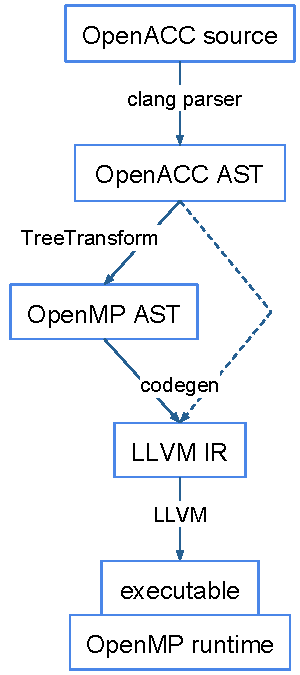
\includegraphics[scale=.65]{projects/2.3.2-Tools/2.3.2.10-PROTEAS-YTUNE/clacc.pdf}}

\end{tabular}

\vspace{-1em}

\begin{enumerate}

\setcounter{enumi}{3}

\item To take advantage of analyses and optimizations at the LLVM IR level,
we are investigating ongoing efforts to develop a parallel LLVM IR, which
clacc could use as an alternative code generation target.

\item To stage our development effort, we are initially implementing clacc
with two simplifications: we are implementing a prescriptive interpretation
of OpenACC to achieve correct behavior, and we are implementing and testing
only within C.  We will extend this implementation with the necessary
analyses and optimizations for a descriptive interpretation and for C++
afterward.  

\item Throughout clacc development, we are continuously integrating the
latest upstream clang/LLVM changes, and we are running and extending the
clang/LLVM test suites to detect regressions and incompatibilities.  We are
also investigating OpenACC benchmarks \cite{specAccel} and validation test
suites \cite{openACCValidationSuite} to ensure correct OpenACC behavior and
good performance.

% \item We will utilize OpenARC, an OpenACC compiler we have developed
% in-house as a research platform for rapidly prototyping cutting-edge
% compiler analyses and optimizations.  After a successful proof-of-concept
% implementation in OpenARC, we will port and harden such compiler techniques
% in clacc.

\end{enumerate}


\paragraph{Recent Progress}

\begin{enumerate}

\item Prototyped the translation of an initial set of OpenACC directives and
clauses to OpenMP.

\item Investigated OpenACC applications, benchmarks, and validation test
suites for use in clacc testing.  Reached out to ECP application teams who
have expressed interest in OpenACC.

\item Initiated clacc design discussions within the clang/LLVM developer
community.

\item Contributed to upstream clang/LLVM a number of fixes and other
improvements to clang attribute and printing support, the clang/LLVM testing
infrastructure, and the OpenMP implementation.

\end{enumerate}


\paragraph{Next Steps}

\begin{enumerate}

\item Complete clacc support for a prescriptive interpretation of OpenACC
for correct behavior, and continue to contribute mutually beneficial
improvements to upstream clang/LLVM as we develop them.

\item Continue clacc design discussions with the clang/LLVM developer
community.

\item Explore applications from ECP teams we have previously contacted.
	
\end{enumerate}
